\documentclass[12pt]{article}

\usepackage{sbc-template}
\usepackage{graphicx,xurl}
\usepackage[brazil]{babel}
\usepackage[utf8]{inputenc}
\usepackage{enumitem,kantlipsum}
\usepackage{amsfonts}
\usepackage{amssymb}
\usepackage{algorithm} 
\usepackage[noend]{algpseudocode}
\usepackage{booktabs}
\usepackage{colortbl}
\usepackage{mathtools}
\usepackage{multirow}
\usepackage{float}
\usepackage[dvipsnames]{xcolor}

\newcommand{\FancyUpArrow}{\textcolor[rgb]{0.0, 0.7, 0.0}{$\blacktriangle$}}
\newcommand{\FancyDownArrow}{\textcolor[rgb]{0.7, 0.0, 0.0}{$\blacktriangledown$}}
\newcommand{\FancyCircle}{\textcolor[rgb]{0.9, 0.9, 0.0}{$\bullet$}}
\definecolor{Gray}{gray}{0.9}
\definecolor{StrongGray}{gray}{0.7}

\sloppy

\title{Análise de Abordagens Distintas na Modelagem de Crescimento de Tumores com EDOs}

\author{Julio Cesar da Silva Rodrigues\inst{1}}

\address{Curso de Graduação em Ciência da Computação\\
         Universidade Federal de São João del-Rei\\
         São João del-Rei -- MG -- Brazil
         \email{julio.csr.271@aluno.ufsj.edu.br}
}

\begin{document} 

\maketitle

\begin{abstract}
    In this work, we present a small comparison between technologies used in the field of computational modeling. Utilizing already consolidated models of tumor growth based on ODEs and delayed ODEs, we implemented such models using a more simplistic approach in the choice of methods and algorithms for parameter estimation and computational simulations. Eventually, we obtain a face to face comparative between the technologies, highlighting similarities, differences, advantages and disadvantages in the application of each tool and the behavior of the associated data.
\end{abstract}

\begin{resumo} 
    Neste trabalho, apresentamos um pequeno comparativo entre tecnologias utilizadas com âmbito da modelagem computacional. Utilizando como base modelos já consolidados de crescimento de tumor baseados em EDOs e EDOs com atraso, implementamos tais modelos utilizando uma abordagem mais simplista na escolha dos métodos e algoritmos para estimação de parâmetros e simulações computacionais. Ao final, obtemos um comparativo entre as tecnologias, destacando similaridades, diferenças, vantagens e desvantagens na aplicação de cada ferramenta e o comportamento dos dados associados.
\end{resumo}

\section{Introdução}

Existe uma etapa essencial do desenvolvimento pré-clínico de drogas na oncologia: a avaliação \emph{in vivo} do efeito antitumoral. Nesta etapa, uma série de experimentos são realizados, nos quais as células tumorais são injetadas em cobaias. Então, os volumes de tumor são mensurados em diferentes momentos ao longo do tempo em todas as cobaias, tratadas como controle (sem aplicação de medicamento) ou com droga ativa. Transcorrida esta etapa, são realizadas uma série de observações para observar possíveis efeitos esperados (e adversos) da droga em relação à ploliferação, atenuação e morte das células cancerígenas.

Simeoni et al. \cite{tu} introduziram e desenvolveram um modelo de crescimento do tumor mamário a partir de estudos em animais (ratos) \emph{in vivo}, estes que poderiam se matematicamente resumidos por um sistema de equações diferenciais ordinárias (EDOs). O modelo e as adaptações provaram ser bastante bem-sucedidos em prever ou modelar crescimento do tumor e eficácia dos tratamentos contra o câncer.

Este trabalho propõe-se à analisar e implementar uma adaptação do modelo de Simeoni proposta por Koziol et al. \cite{my}, esta que utiliza sistema de EDOs com atraso. O foco principal neste ponto, é utilizar algoritmos e métodos do âmbito da modelagem computacional alheios aqueles utilizados no artigo analisado. O propósito central em tal abordagem é estudar as possíveis semelhanças e diferenças, vantagens e desvantagens, provocadas pela utilização de ferramentas distintas para estimação de parâmetros e simulação de modelos computacionais.

Este artigo está organizado da seguinte forma: a Seção \ref{sec:1} o referencial teórico, destacando conceitos fundamentais; a Seção \ref{edo:2} são descritos os modelos computacionais implementados; na Seção \ref{sec:3} é descrita a metodologia de desenvolvimento empregada; a Seção \ref{sec:4} apresenta uma análise sobre os resultados obtidos; a Seção \ref{sec:5} discute conclusões deste trabalho e apresenta questões a serem consideradas em possíveis trabalhos futuros.

\section{Referencial Teórico} \label{sec:1}

Existem diversas formas de formular um modelo que seja capaz de simular com precisão as observações reais realizadas no desenvolvimento e aplicação de medicamentos. Uma destas formas utiliza das EDOs, modelos matemáticos capazes de simular o comportamento de variáveis ao longo do tempo (não se aplica ao espaço).

Além de aplicarem EDOs na formulação de seus modelos, os artigos até então citados consideram algumas hipóteses e sofrem de algumas limitações que serão discutidas nesta seção. A principal hipótese é de sempre existe um atraso de tempo até que a medicação aplicada inicie seu efeito imunoterapêutico. Como principal limitação, tais modelos não consideram um limite superior na mensuração do tamanho de tumores. Existem limites não só físicos, mas também biológicos que demonstram que tal fator deve ser considerado na maioria dos casos de estudo no campo.

Em relação aos métodos e algoritmos do âmbito da modelagem computacional utilizados neste trabalho, o Runge-Kutta de 4ª ordem é um dos mais importantes \emph{solvers} iterativos, utilizado para a resolução numérica de soluções de equações diferenciais ordinárias, pertencente à família de métodos de Runge–Kutta \cite{BUTCHER1996247} iterativos implícitos e explícitos.

Por fim, o algoritmo de evolução diferencial (DE) \cite{article} é um método heurístico, que usufrui de vários conceitos dos algoritmos genéticos, cujo objetivo é solucionar problemas de otimização contínua. É um algoritmo que trabalha com busca estocástica, robusto a mínimos locais, eficaz em otimização numérica para busca de uma solução ótima global.

\section{Modelos Propostos} \label{sec:2}

Nesta seção, serão discutidos em detalhes os modelos apresentados pelo artigo proposto, explanando as informações mais relevantes como parâmetros, variáveis, entre outros. No artigo analisado, os autores apresentam duas formulações para modelagem de crescimento de tumores, a primeira abordada com EDOs (Equações Diferenciais Ordinárias), e outra baseada em EDOs com atraso.

\subsection{Modelo de Simeoni}

Simeoni et al. propõem um modelo baseado em \(N\) compartimentos subsequentes atenuadores de células, inibindo suas proliferações e danificando-as até a morte, conforme a aplicação de medicamentos anticancerígenos. Geralmente, o número de compartimentos é escolhido de forma arbitrária, levando em consideração por exemplo, o modelo de EDOs. A Figura \ref{fig:map1} descreve de forma esquemática o modelo: 

\begin{figure}[H]
    \centering
    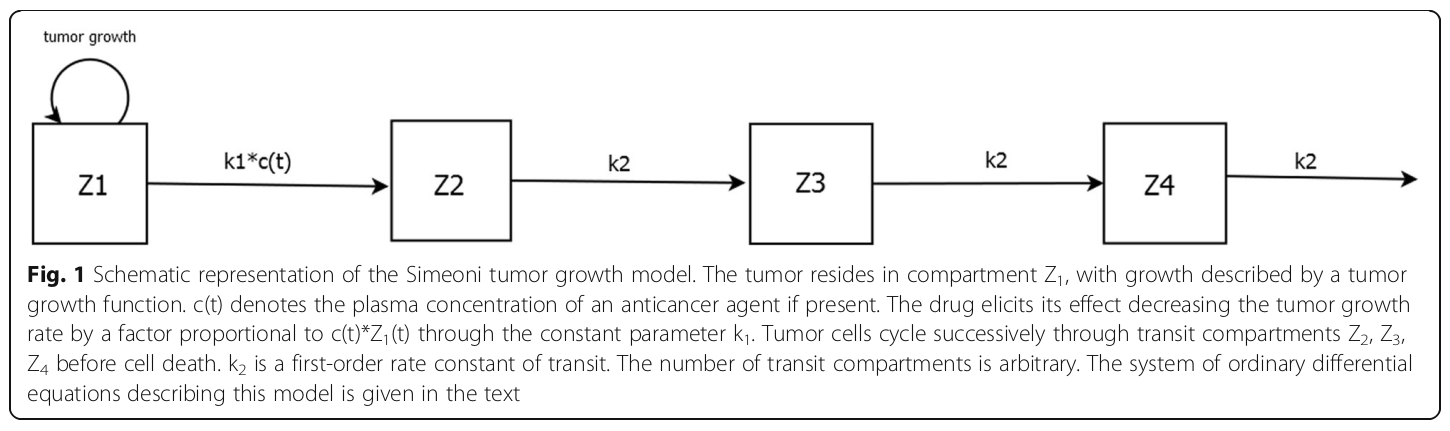
\includegraphics[width=1\textwidth]{pic/simeoni.png}
    \hspace*{15pt}\hbox{\small Fonte:\thinspace{(Simeoni et al., 2004, Pág. 2)}}\\
    \label{fig:map1}
\end{figure}

A função de crescimento de tumor e a concentração de células cancerígenas não atenuadas ao longo do tempo no compartimento fonte (\emph{Z1}), são exibidas em detalhes na equação \ref{eq:1} e na EDO \ref{edo:1}:

\begin{equation} \label{eq:1}
    TGF(t) = \frac{\lambda_0 \cdot Z_1(t)}{\left[1 + \left(\frac{\lambda_0}{\lambda_1} \cdot V(t)\right)^\Psi\right]^{\frac{1}{\Psi}}},
\end{equation}

\begin{equation} \label{edo:1}
    \frac{dZ_1(t)}{dt} = TGF(t) - k_1 \cdot c(t) \cdot Z_1(t),
\end{equation}

onde:

\begin{itemize}
    \setlength{\itemsep}{10pt}
    \item \emph{Z1(t)}: Concentração de células cancerígenas não atenuadas ao longo do tempo;
    \item \emph{V(t)}: Volume do tumor ao longo do tempo;
    \item \(\lambda_0\): Taxa de crescimento exponencial;
    \item \(\lambda_1\): Taxa de crescimento linear;
    \item \(\Psi\): Aproximação do sistema de comutação original.
    \item \(k_1\): Taxa de transição para atenuação;
    \item \emph{c(t)}: Aplicação de doses de medicamento anti-cancerígeno ao longo do tempo.
\end{itemize}

A transição entre compartimentos e atenuação de células cancerígenas, inibindo suas proriferações e eventualmente causando suas mortes são formuladas em detalhes com as EDOS \ref{edo:2}, \ref{edo:3} e \ref{edo:4}:

\begin{equation} \label{edo:2}
    \frac{dZ_2(t)}{dt} = k_1 \cdot c(t) \cdot Z_1(t) - k_2 \cdot Z_2(t),
\end{equation}

\begin{equation} \label{edo:3}
    \frac{dZ_3(t)}{dt} = k_2 \cdot Z_2(t) - k_2 \cdot Z_3(t),
\end{equation}

\begin{equation} \label{edo:4}
    \frac{dZ_4(t)}{dt} = k_2 \cdot Z_3(t) - k_2 \cdot Z_4(t),
\end{equation}

onde:

\begin{itemize}
    \setlength{\itemsep}{10pt}
    \item \emph{Zi(t)}: Concentração de células atenuadas no estágio \emph{i} ao longo do tempo;
    \item \(k_2\): Taxa de transição entre estados de atenuação (até eventual morte).
\end{itemize}

\subsection{Modelo de Koziol}

Simeoni et al. propõem um modelo baseado no estudo do modelo de Simeoni, condensando os \(N\) compartimentos subsequentes atenuadores de células em apenas um único compartimento \emph{Z2}. Tal modelo trata as transições das células com EDOs com atraso, aplicando \emph{N} passos de tempo para o processo de atenuação. A Figura \ref{fig:map2} descreve de forma esquemática o modelo:

\begin{figure}[H]
    \centering
    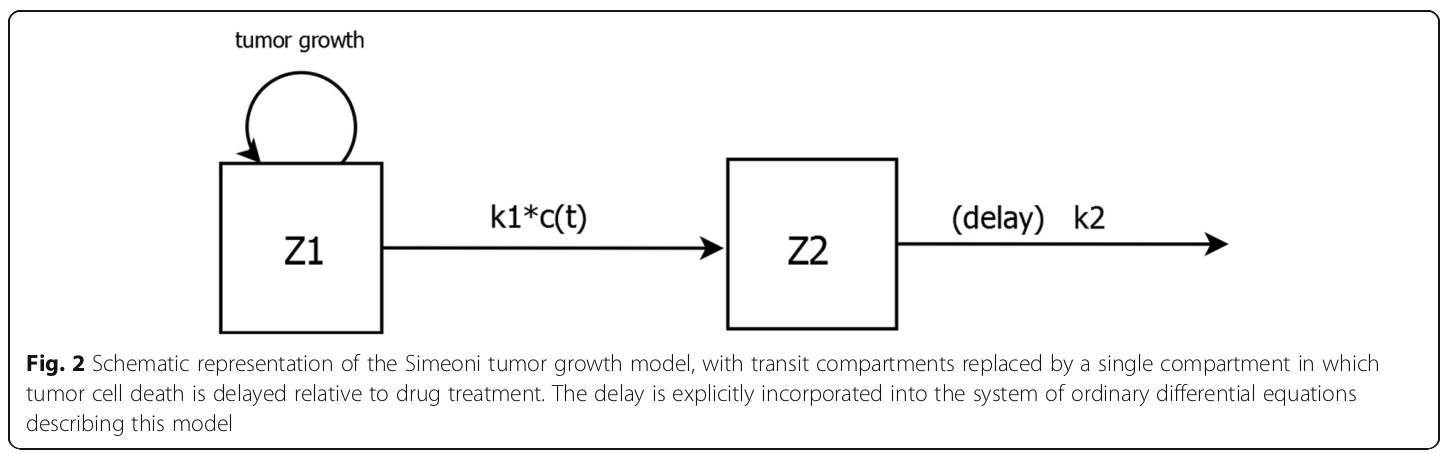
\includegraphics[width=1\textwidth]{pic/proposal.png}
    \hspace*{15pt}\hbox{\small Fonte:\thinspace{(Koziol et al., 2020, Pág. 2)}}\\
    \label{fig:map2}
\end{figure}

Enquanto a formulação do compartimento das células cancerígenas não atenuadas \emph{Z1} continua o mesmo, a aplicação de atenuação nas células no compartimento \emph{Z2} é ligeiramente distinta, exibida em detalhes na EDO \ref{edo:5}:

\begin{equation} \label{edo:5}
    \frac{dZ_2(t)}{dt} = k_1 \cdot c(t) \cdot Z_1(t) - k_2 \cdot delay(Z_2, t_2),
\end{equation}

onde:

\begin{itemize}
    \setlength{\itemsep}{10pt}
    \item \(delay(Z_2, t_2)\) = \(Z2(t - t_2)\);
    \item \(t_2\): Atraso de tempo antes da eliminação.
\end{itemize}

\section{Metodologia} \label{sec:3}

Nesta seção, serão discutidas questões sobre a metodologia empregada no desenvolvimento, incluindo mas não limitado à, bases de dados e tecnologias utilizadas e detalhes gerais de implementação, incluindo métodos, simulações e testes. É importante citar de antemão, que todo o desenvolvimento deste trabalho foi realizado utilizando a linguagem Python\footnotemark \hspace{0.1cm}em conjunto com as bibliotecas Matplotlib\footnotemark, pandas\footnotemark e SciPy\footnotemark. A implementação encontra-se disponível publicamente em \url{https://github.com/juliorodrigues07/tumor_growth}.

\footnotetext[1]{\scriptsize Mais informações em: \url{https://www.python.org/}}
\footnotetext[2]{\scriptsize Mais informações em: \url{https://matplotlib.org/}}
\footnotetext[3]{\scriptsize Mais informações em: \url{https://pandas.pydata.org/}}
\footnotetext[4]{\scriptsize Mais informações em: \url{https://scipy.org/}}

\subsection{Base de Dados} \label{subsec:1}

Realizada a requisição aos autores da base de dados utilizada nas fases experimentais descritas no artigo analisado, obtive dois arquivos contendo dados sobre observações realizadas em cada uma das 40 cobaias analisadas.

Segundo informações extraídas do próprio artigo, existem várias métricas relacionadas a tamanho e volume mensuradas em 40 ratos. Destes, apenas 19 receberam um tratamento com uma dose única de \emph{cisplatin} (agente imunoterapêutico) no início do experimento, enquanto o restante não recebeu quaisquer tipos de tratamento para efeitos comparativos. Além disso, todos os animais aparentavam estar saudáveis no primeiro dia, com volume de tumor mensurado abaixo a determinado limiar.

Em ambas as bases de dados (animais tratados e de controle), podemos observar um total de 8 informações para cada observação. São estas:

\begin{itemize}
    \setlength{\itemsep}{10pt}
    \item DAY: Total de dias transcorridos desde o início do experimento;
    \item L (\emph{Length}): Comprimento do tumor (em \emph{mm});
    \item W (\emph{Width}): Largura do tumor;
    \item H (\emph{Height}): Altura do tumor;
    \item \{Vol1, Vol2, Vol3\footnotemark\}: Métricas distintas dos volumes de tumores;
    \item ID: Identificação da cobaia.
\end{itemize}

\footnotetext[5]{\scriptsize{Pode ser calculado como: \(Vol3 = \frac{L \times W^2}{2}\)}}

Como não existem informações explícitas sobre a base de dados, indicando se existem colunas que correspondem à quantidade de células em cada compartimento, foi realizada uma adaptação para executar os processos de estimação de parâmetros e as simulações. 

É discutido no artigo, que o volume total do tumor pode ser obtido como a soma da concentração de células em cada um dos compartimentos. Além disso, a métrica \emph{Vol3} depende diretamente dos valores das métricas \emph{L} e \emph{W}, e a condição
\begin{equation*}
    L > W,
\end{equation*}
sempre é satisfeita, considerou-se que a coluna \emph{L} corresponde ao número de células contidas no compartimento \emph{Z1}, e a coluna \emph{W} corresponde à quantidade de células contidas no compartimento \emph{Z2}. Logo, as colunas restantes com exceção das que identificam o dia da observação e a cobaia (\emph{DAY} e \emph{ID}), não foram utilizadas em nenhum momento no desenvolvimento deste trabalho.

\subsection{Implementação}

No artigo analisado, os autores utilizaram uma série de ferramentas sofisticas no âmbito da modelagem computacional para alcançar os resultados desejados. Utilizou-se o modelo NLME\footnotemark \hspace{0.1cm} para ajustar as curvas de crescimento, otimizando valores para população inicial e variabilidade interindividual.

\footnotetext[6]{\scriptsize{Nonlinear Mixed Effects}}

Além disto, foi utilizada a \emph{suite} de programas Monolix 2019R1\footnotemark, voltada para utilização em farmacometria, cujas licenças podem ser obtidas gratuitamente para uso acadêmico. Esta ferramenta foi empregada com o propósito de estimar parâmetros, aplicando uma algoritmo baseado em SAEM\footnotemark, estimando os parâmetros do modelo pela técnica de máxima verossimilhança.

\footnotetext[7]{\scriptsize{Mais informações em: \url{https://lixoft.com/products/monolix/}}}
\footnotetext[8]{\scriptsize{Stochastic Approximation Expectation Maximization}}

Neste trabalho, foi construída uma implementação para estimar vários dos parâmetros do modelo de EDOs com atraso proposto, utilizando algoritmos considerados como clássicos no âmbito da modelagem computacional. O algoritmo em questão é baseado em evolução diferencial, e os parâmetros a serem estimados foram os seguintes:

\begin{itemize}
    \setlength{\itemsep}{10pt}
    \item \(\lambda_0\): Taxa de crescimento exponencial;
    \item \(\lambda_1\): Taxa de crescimento linear;
    \item \(k_1\): Taxa de transição para atenuação;
    \item \(k_2\): Taxa de transição entre estados de atenuação (até eventual morte).
\end{itemize}

Na formulação da EDO com atraso, foi utilizado um \emph{delay} de dois passos de tempo, assim como proposto no artigo analisado. Portanto, a concentração de células atenuadas no compartimento \emph{Z2} em \(t = 0\) e \(t = 1\) é nula na estimação de parâmetros e simulação do modelo. Uma lista contendo as concentrações das respectivas células nos dois passos de tempo anteriores é mantida, sempre atualizada a cada iteração. A partir de \(t = 2\), é incluída a concentração de \emph{Z2} em \(t = t - 2\) nas estimações e simulações.    

Para estimar os parâmetros, utilizamos como ponto de partida as base de dados recém mencionadas. Neste ponto, analisando o arquivo contendo dados sobre as cobaias não tratadas como exemplo, tais parâmetros foram estimados para cada cobaia individualmente. É importante citar que o parâmetro \(\Psi\) não foi estimado em nenhum momento. Apenas foi atribuída uma constante \(\Psi=20\) como explanado no trabalho de Simeoni et al. (Simeoni et al., 2004, Pág. 2), alegando que tal valor permite que o crescimento do sistema transite de primeira ordem para ordem zero de forma acentuada o suficiente.

Foram armazenadas as taxas para cada subconjunto de dados em uma lista, cujo tamanho é a quantidade de cobaias contidas na base de dados. Ao final, calcula-se a média entre todos os subconjuntos de soluções obtidas para os dados de cada cobaia, resultando na solução final com parâmetros estimados. O mesmo processo é executado para a base de animais tratados no início do experimento, obtendo dois conjuntos de parâmetros para casos sem e com tratamento.

Após a estimação dos parâmetros, foram executadas simulações com os mesmos atribuídos, com o intuito de verificar o comportamento do crescimento de tumor mamário em cada cobaia das bases de dados. Além disso, os dados experimentais também são exibidos no gráfico como pontos.

O objetivo em planarizar estes dados, é realizar um comparativo com as simulações apresentadas no artigo analisado, identificando as possíveis semelhanças e disparidades no crescimento do volume de tumores. Com isto, obtemos uma base inicial para comparar o nível de ajuste e satisfação dos resultados obtidos entre as ferramentas:

\begin{itemize}
    \setlength{\itemsep}{10pt}
    \item NLME x RK4\footnotemark;
    \item SAEM x Evolução Diferencial.
\end{itemize}

\footnotetext[9]{\scriptsize{Método Runge-Kutta de 4ª ordem}}

\section{Resultados} \label{sec:4}

Nesta seção, serão discutidos brevemente alguns dos resultados obtidos no processo de estimação dos parâmetros, simulações do modelo e análises comparativas com dados experimentais.

\subsection{Estimação dos Parâmetros}

Nas Figuras \ref{fig:map3} e \ref{fig:map4} são exibidos os gráficos de evolução do erro no ajuste de parâmetros executado com o algoritmo de evolução diferencial. Os gráficos correspondem somente ao ajuste para uma cobaia sem tratamento e uma cobaia que recebeu tratamento no início do experimento, respectivamente.

\begin{figure}[H]
    \centering
    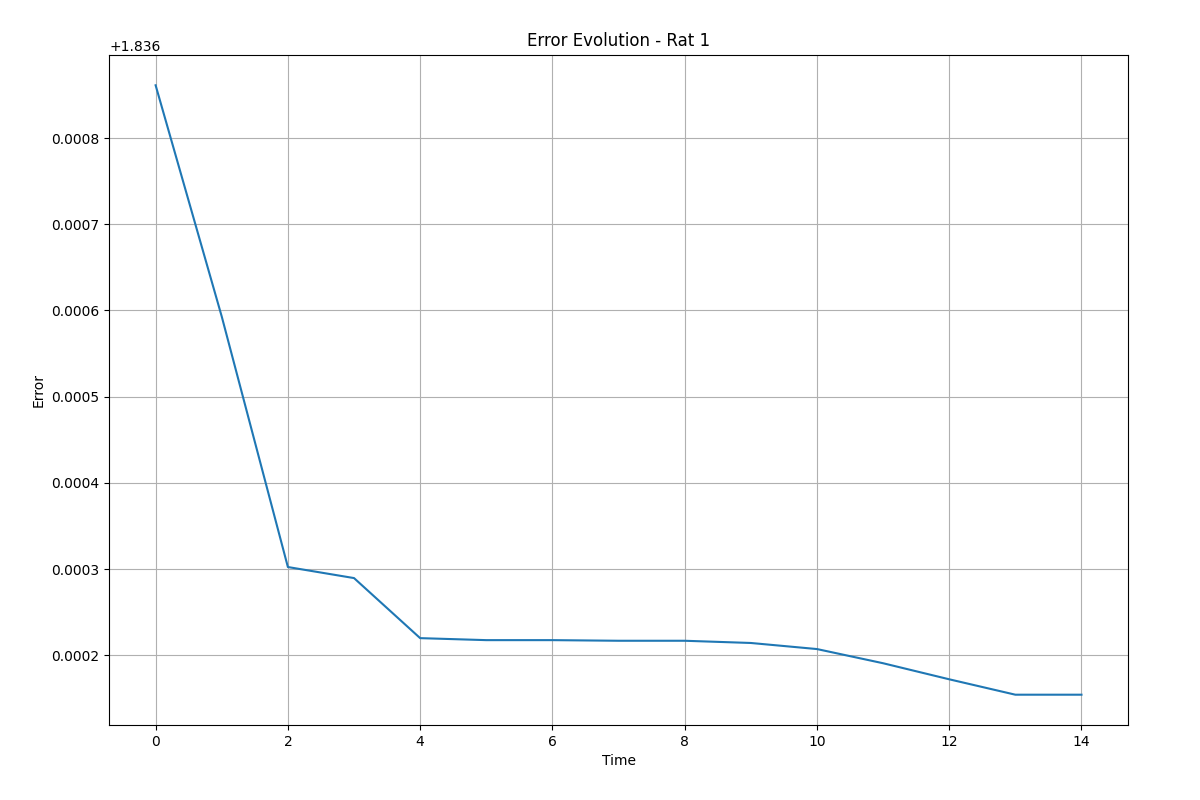
\includegraphics[width=0.85\textwidth]{pic/error_no.png}
    \caption{Ajuste de parâmetros para cobaia 1 sem tratamento}
    \label{fig:map3}
\end{figure}

\begin{figure}[H]
    \centering
    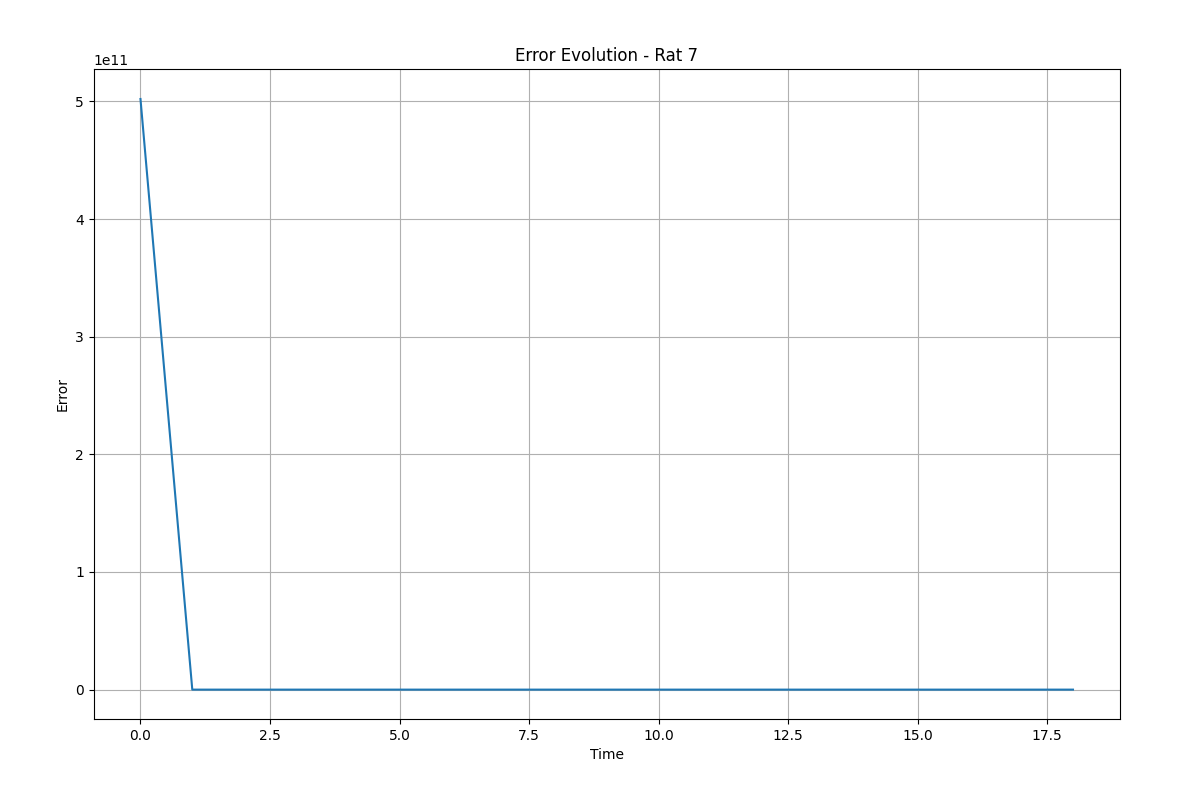
\includegraphics[width=0.85\textwidth]{pic/error_yes.png}
    \caption{Ajuste de parâmetros para cobaia 7 sem tratamento}
    \label{fig:map4}
\end{figure}

É importante citar que no processo de estimação dos parâmetros, os limites inferior e superior foram fixados no intervalo [0.01, 1] para todos os parâmetros. O resultados obtidos ao final da execução do algoritmo de evolução diferencial para os dados de ambos os tipos de cobaias são sumarizados na Tabela \ref{tab:exampleTab1}.

\begin{table}[H]
    \centering
    \caption{Parâmetros estimados para cada tipo de cobaia}
    \label{tab:exampleTab1}
    \vspace{0.2cm}
    \resizebox{.6\columnwidth}{!}{
    \begin{tabular}{c|c|c}
        \hline
        \textbf{Parâmetro} & \textbf{Tratadas}  & \textbf{Não Tratadas}\\
        \hline
        \(\lambda_0\) & 0,02867228 & 0,55265251\\
        \(\lambda_1\) & 0,1863795 & 0,99993298\\
        \(k_1\) & 0,55193695 & 0,52167446\\
        \(k_2\) & 0,8883638 & 0,01000157\\
        \hline 
    \end{tabular}
    }
\end{table}

Podemos observar uma nítida disparidade nos parâmetros \(\lambda\) entre as bases de dados, com as taxas de crescimento exponencial e linear estimadas para a base de cobaias não tratadas relativamente maiores às da base de cobaias tratadas. Tal observação condiz com o esperado, já que presume-se que cobaias não tratadas possuam crescimento de tumor acelerado em relação à cobaias que receberam medicação, mesmo que esta seja uma dose única e pequena ao início do experimento.

Por fim, enquantos os valores estimados para \(k_1\) se mantém próximos, indicando uma taxa similar de proriferação de células cancerígenas, voltamos a observar disparidades para o parâmetro \(k_2\). Todavia, encontra-se um resultado que encaixa-se com as expectativas, indicando que células transitam mais rapidamente entre estados de atenuação em cobaias que receberam tratamento, indicando uma taxa maior para \(k_2\).

\subsection{Simulações}

Embora os parâmetros estimados até o momento se apresentem condizentes com os resultados esperados, as simulações executadas exibem um comportamento de crescimento de tumor distintas em geral daquelas apresentadas no artigo analisado. Acredita-se que pelo menos parte destes resultados errôneos pode ser atribuída à possível má interpretação da base de dados, e a adaptação já mencionada na Subseção \ref{subsec:1} para obter o número de células em cada compartimento observado nos experimentos.

No artigo analisado, somente são realizadas simulações com o modelo de EDOs com atraso para o caso de cobaias que receberam tratamento no início do experimento. Logo, neste trabalho somente serão apresentadas as simulações que se encaixam neste cenário. Para condensar a visualização das simulações, foram selecionadas apenas as correspondentes às 8 primeiras cobaias que receberam tratamento.

Observando as Figuras \ref{fig:map5} e \ref{fig:map6}, que correspondem respectivamente, às simulações do artigo analisado e do presente trabalho, podemos perceber o comportamento totalmente atípico entre as simulações. Enquanto as simulações apresentadas no artigo conseguem se aproximar com certa precisão dos dados experimentais, as simulações deste trabalho sequer conseguem acompanhar parte dos padrões.

\begin{figure}[ht]
    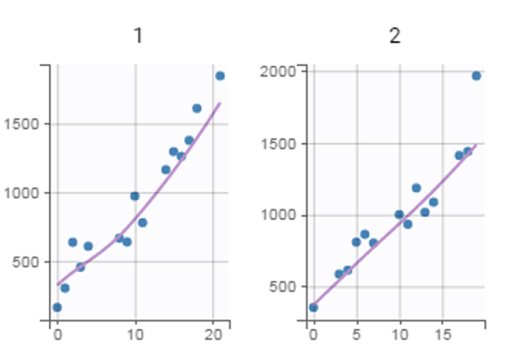
\includegraphics[width=0.5\textwidth]{pic/1.png}
    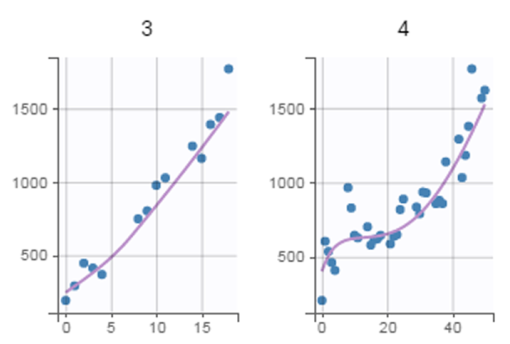
\includegraphics[width=0.5\textwidth]{pic/2.png}
    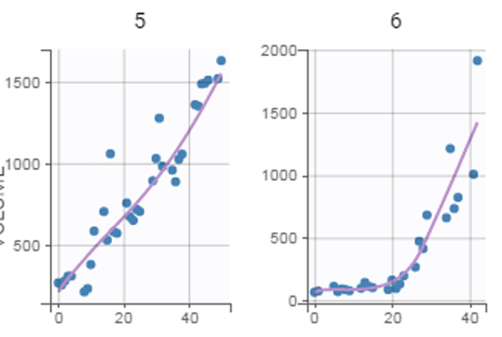
\includegraphics[width=0.5\textwidth]{pic/3.png}
    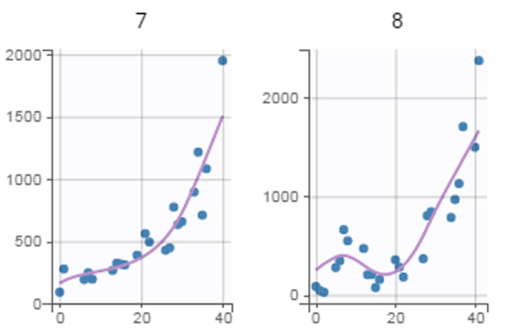
\includegraphics[width=0.5\textwidth]{pic/4.png}
    \hspace*{15pt}\hbox{\scriptsize Fonte:\thinspace{\small\itshape \scriptsize{(Koziol et al., 2020, Pág. 8)}}}\\
    \caption{Simulações com NMLE}
    \label{fig:map5}
\end{figure}

\begin{figure}[ht]
    \centering
    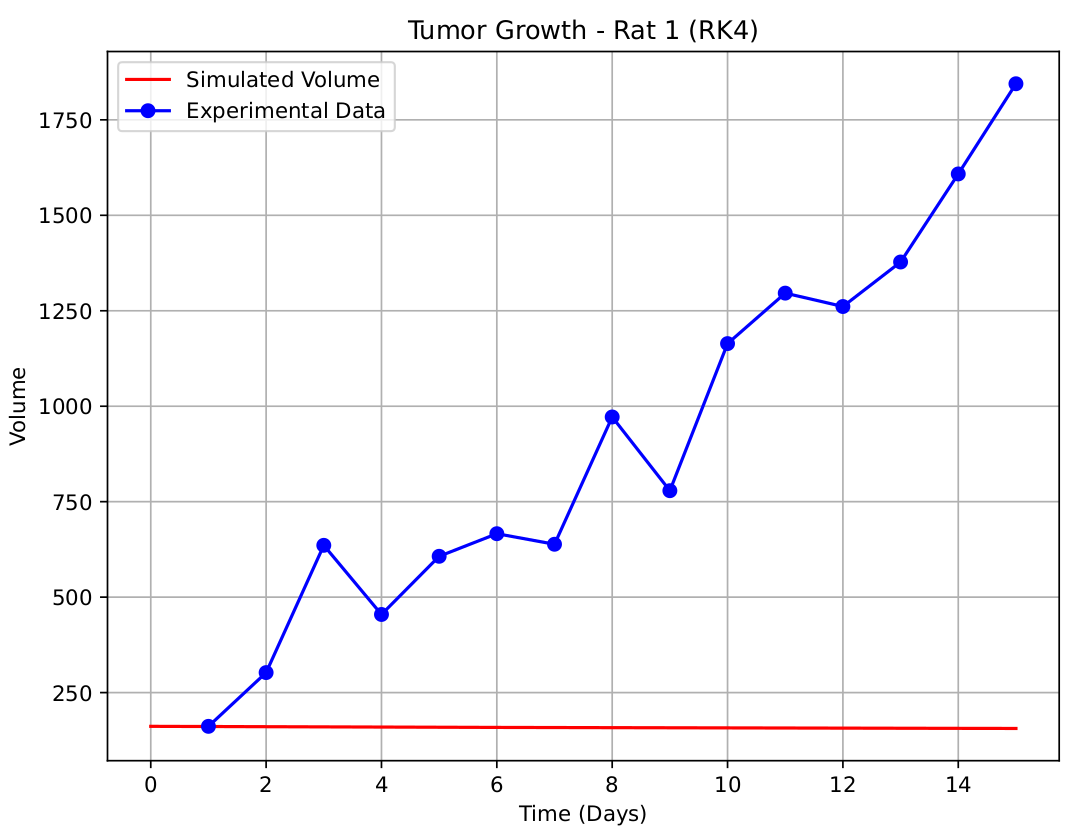
\includegraphics[width=7.3cm,height=6cm]{pic/a.png}
    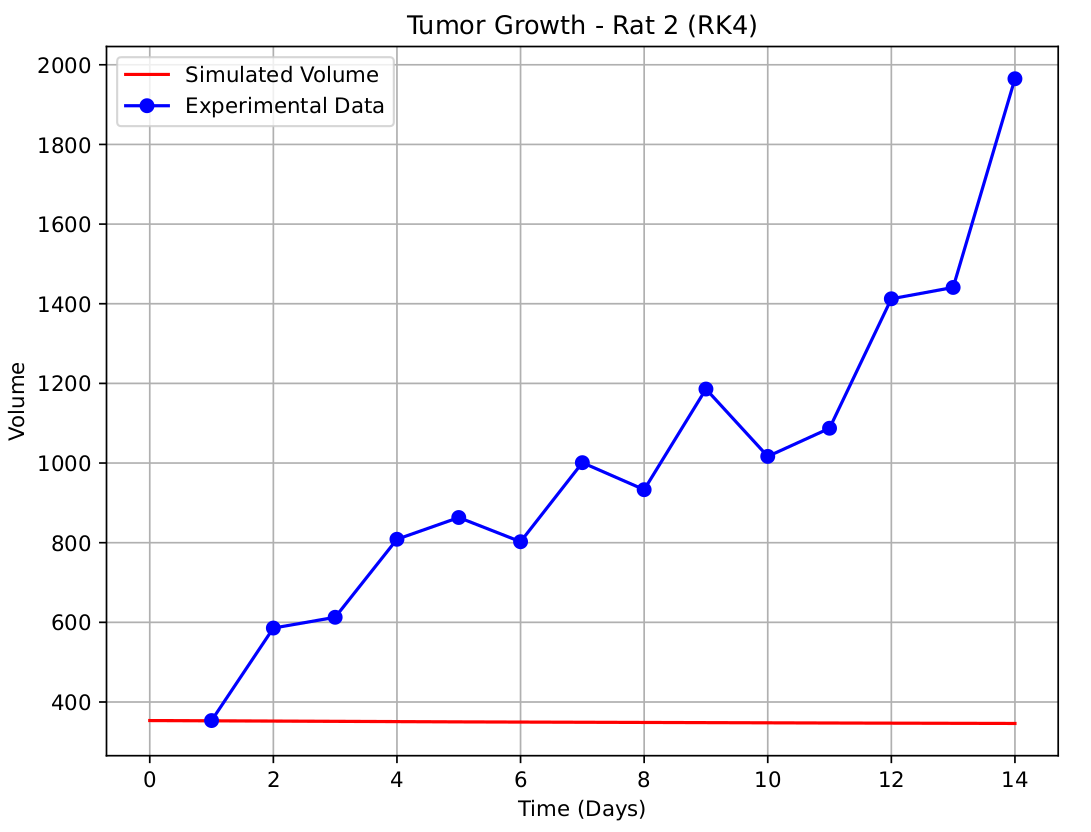
\includegraphics[width=7.3cm,height=6cm]{pic/b.png}
    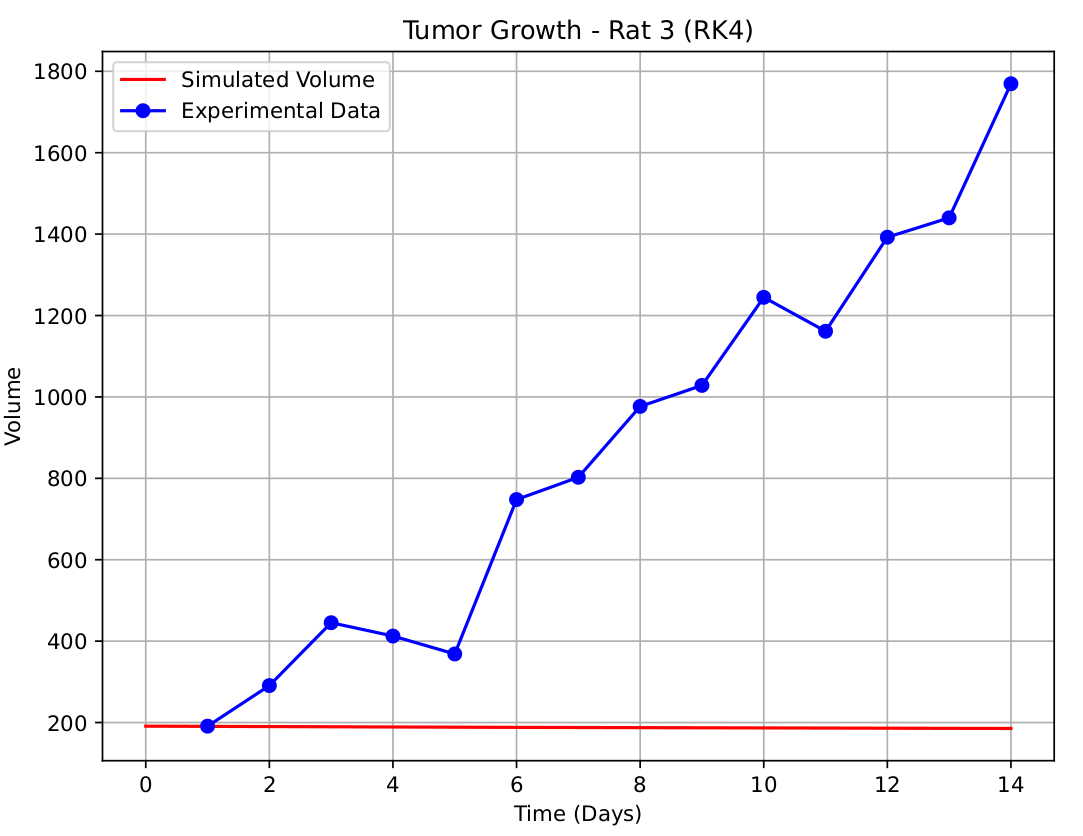
\includegraphics[width=7.3cm,height=6cm]{pic/c.png}
    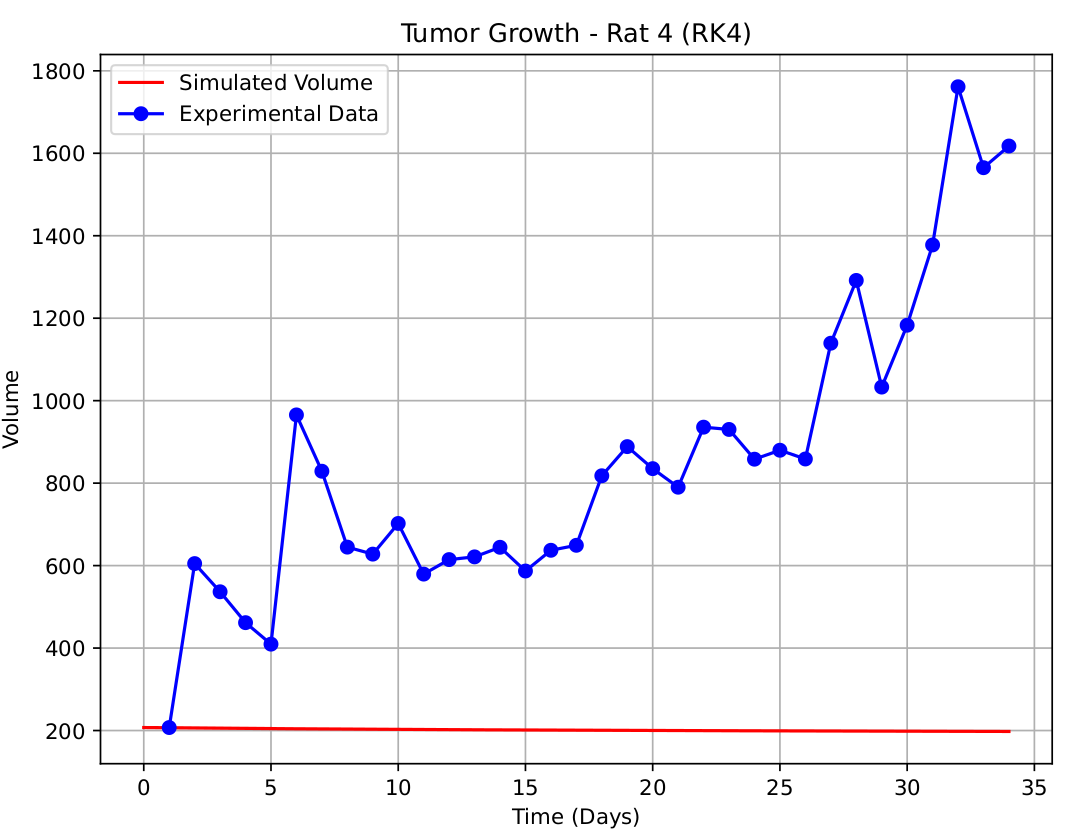
\includegraphics[width=7.3cm,height=6cm]{pic/d.png}
\end{figure}

\begin{figure}[H]
    \centering
    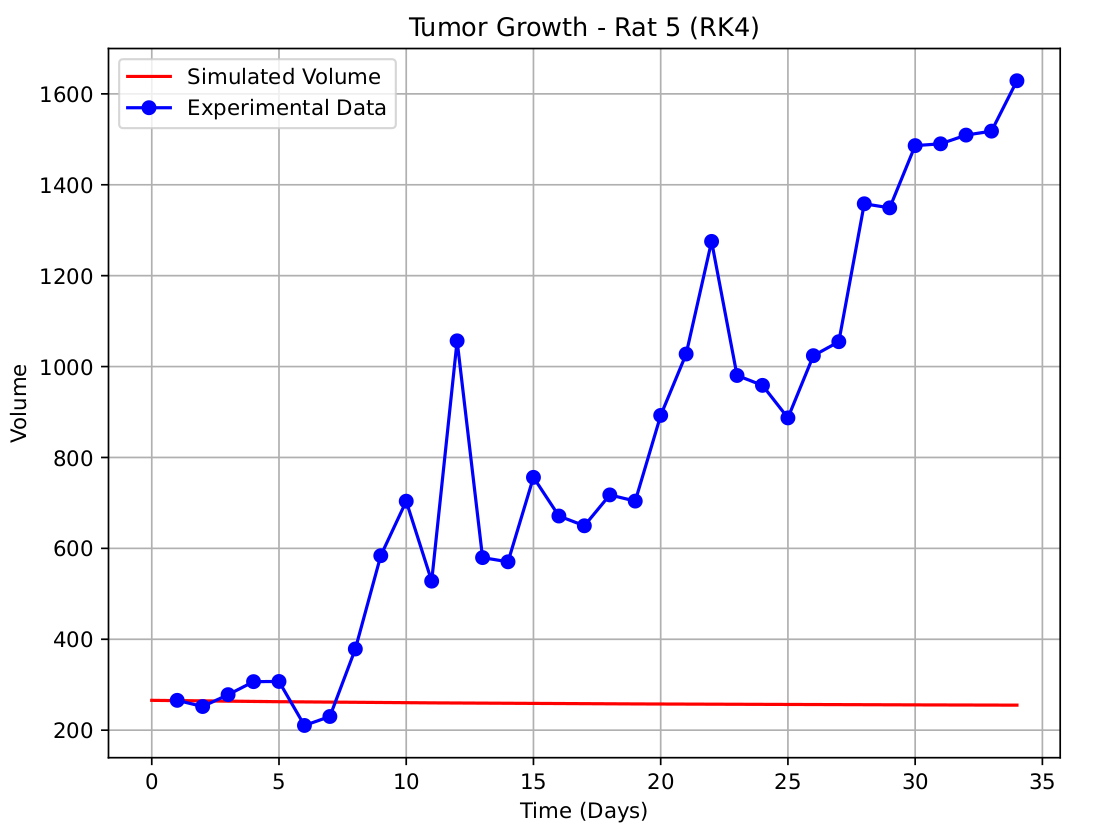
\includegraphics[width=7.3cm,height=6cm]{pic/e.png}
    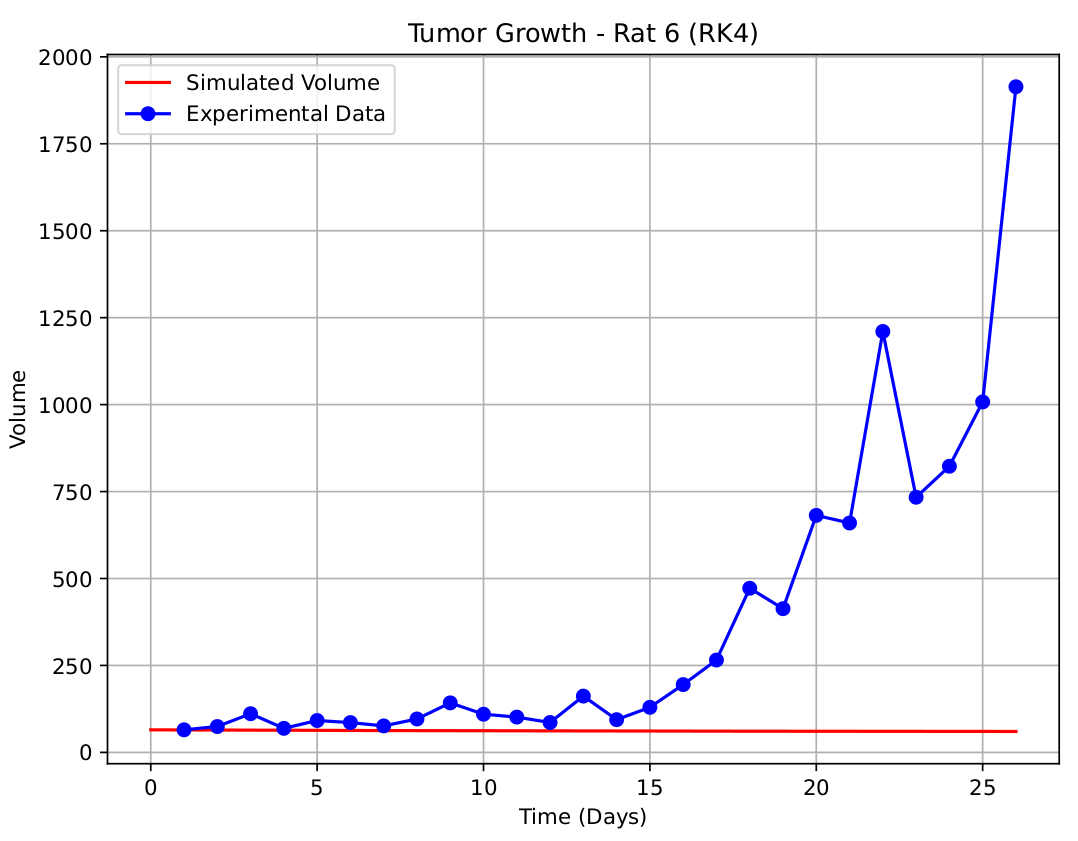
\includegraphics[width=7.3cm,height=6cm]{pic/f.png}
    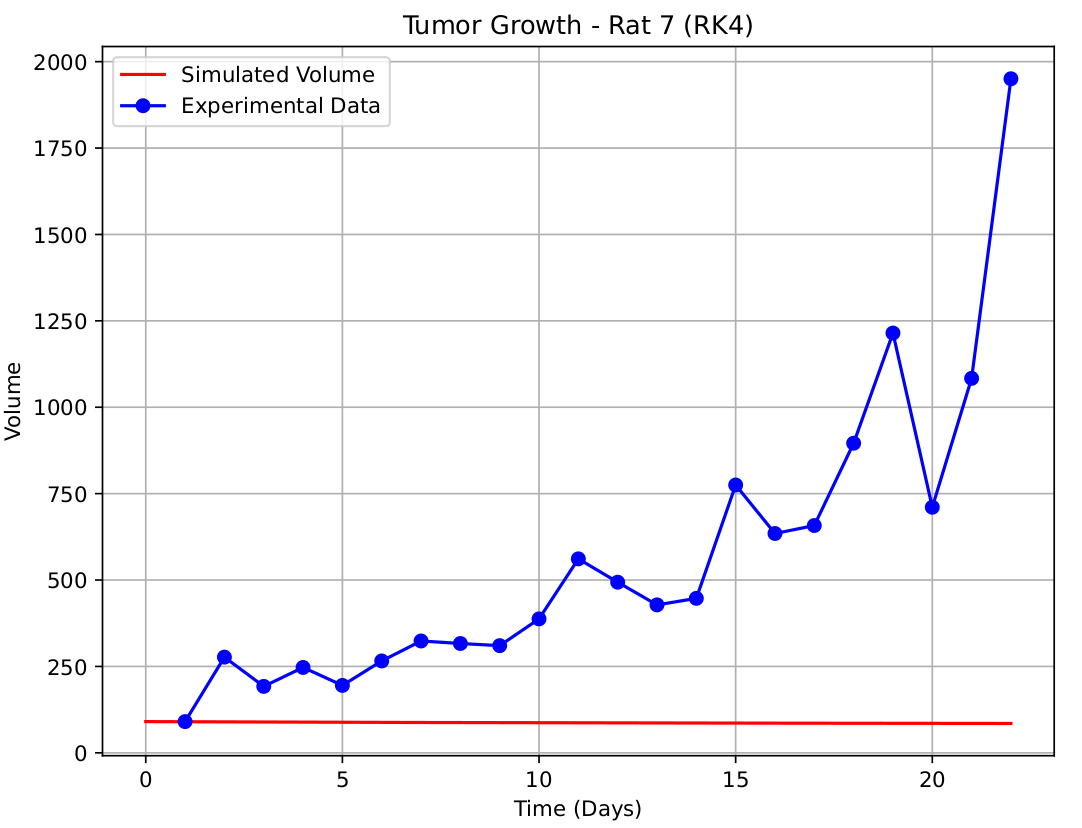
\includegraphics[width=7.3cm,height=6cm]{pic/g.png}
    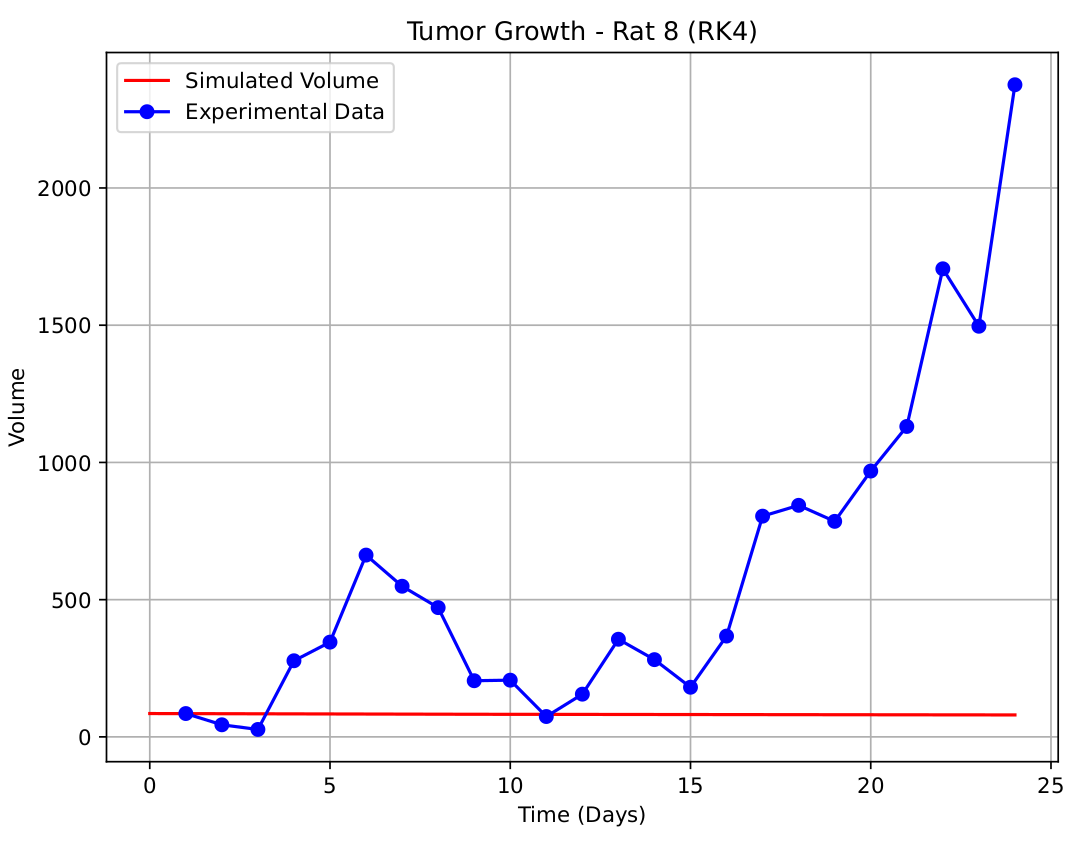
\includegraphics[width=7.3cm,height=6cm]{pic/h.png}
    \caption{Simulações com RK4}
    \label{fig:map6}
\end{figure}

No geral as simulações da Figura \ref{fig:map6} se resumem a crescimentos ou decréscimos constantes e completamente suaves no volume dos tumores. Embora a utilização do método RK4 possivelmente não seja a mais adequada neste cenário, considerando o NMLE aplicado no artigo, resultados tão distantes nos levam a considerar que podem existir erros de implementação, seja na manipulação e adaptação das bases de dados, ou no sistema de EDOs aplicado nas simulações.

Por fim, foram executadas também simulações para cobaias que não receberam tratamento, e o resultado novamente se mostrou completamente alheio às simulações apresentadas no artigo. Além disto, tais simulações também foram executadas realizando alterações nos parâmetros dentro dos limites de estimação, operações que não provocaram nenhuma alteração significativa no comportamento de volume de tumor comparadas às simulações observadas no artigo. 

\section{Considerações Finais} \label{sec:5}

Neste trabalho, foi apresentado uma metodologia distinta e simplista na abordagem de estimação de parâmetros e simulações de modelos de EDOs. Embora possivelmente existam erros na implementação descrita, podemos observar superficialmente a diferença na aplicação de ferramentas do âmbito da modelagem computacional, estas que quando mais sofisticadas, podem prover resultados mais condizentes com dados reais a um custo computacional possivelmente menor ou maior.

Como trabalhos futuros, podemos inicialmente nos limitar à corrigir os obstáculos encontrados no desenvolvimento trabalho, conduzindo um melhor estudo da base de dados, identificando de forma precisa quais informações estão disponíveis. Além disso, podemos testar outros algoritmos de estimação de parâmetros e simulações, aplicar ajuste fino de hiperparâmetros, realizando um comparativo entre si ao final para identificar as semelhanças, diferenças, vantagens e desvantagens entre cada um destes.

\footnotesize
\bibliographystyle{sbc}
\bibliography{sbc-template}
\noindent Repositório com implementações de métodos e modelos de Alexandre Bittencourt Pigozzo: \url{https://github.com/alexbprr/ComputationalModeling}\\

\noindent Material disponível no portal didático na disciplina de Introdução à Modelagem Computacional.

\end{document}